\documentclass{beamer}

\mode<presentation>
{
  \usetheme{Singapore}
  \usecolortheme{default}
  \usefonttheme{default}
  \setbeamertemplate{navigation symbols}{}
  \setbeamertemplate{caption}[numbered]
}

\usepackage[frenchb]{babel}
\usepackage[T1]{fontenc}
\usepackage[utf8]{inputenc}
\usepackage{tikz-qtree}
\usepackage[thinlines]{easytable}
\usetikzlibrary{arrows}

\title{La Voix des Abysses :\\Soutenance de projet long}
\author{Nicolas Descouens, Louis Vignier}
\institute{CentraleSupélec}

\AtBeginSection[]
{
  \begin{frame}
  \frametitle{Sommaire}
  \tableofcontents[currentsection]
  \end{frame}
}

\begin{document}

\begin{frame}
  \titlepage
\end{frame}

\begin{frame}{Plan}
  \tableofcontents
\end{frame}

\section{Introduction}

\subsection{Démarrage du projet}

\begin{frame}{Point de départ}
    \centering
    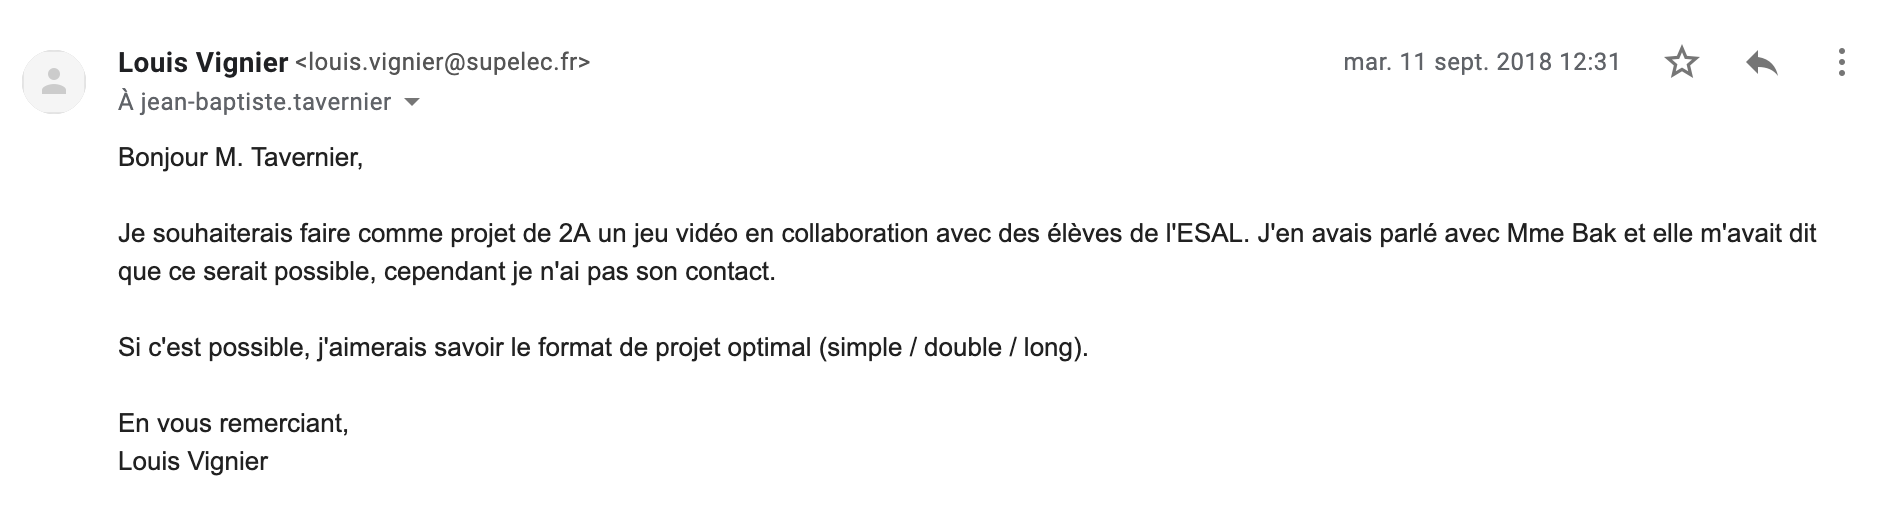
\includegraphics[width=10cm]{assets/debut1}
    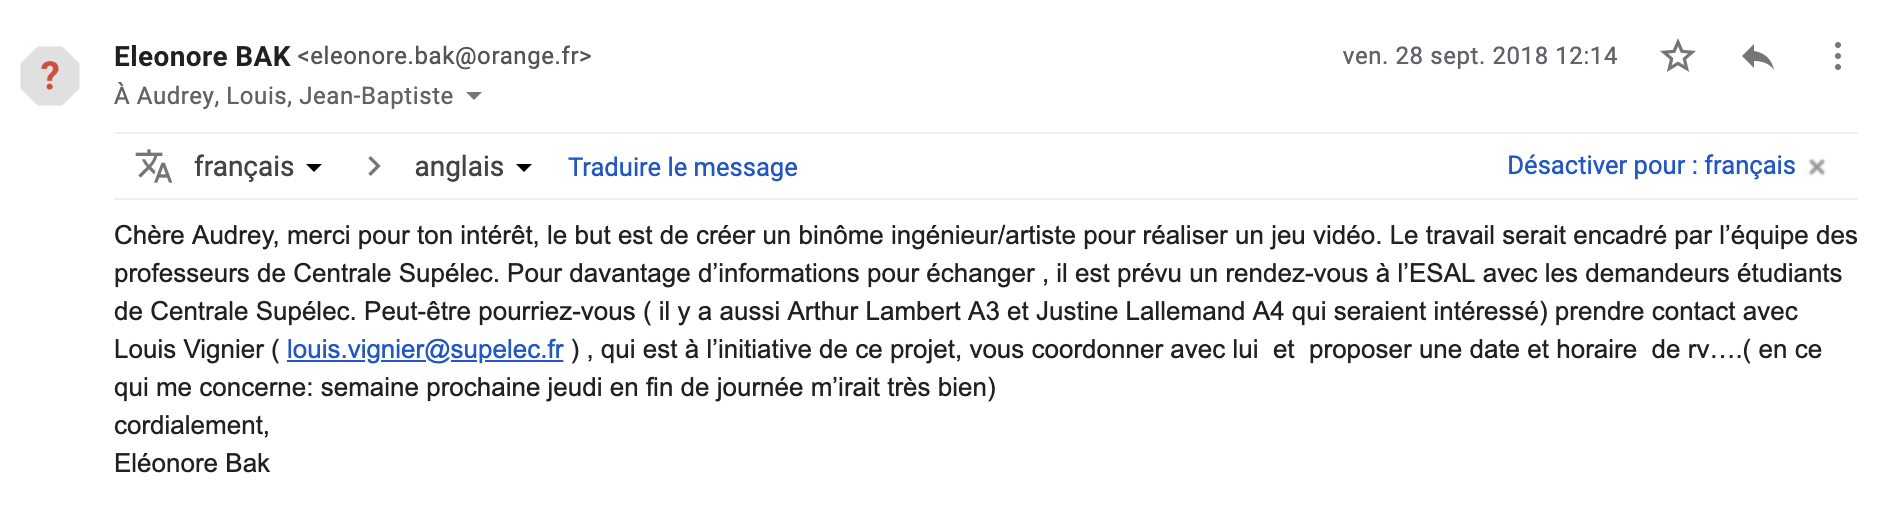
\includegraphics[width=10cm]{assets/debut2}
\end{frame}

\begin{frame}{Équipe}
    \begin{itemize}
        \item CentraleSupélec
        \begin{itemize}
            \item Nicolas Descouens
            \item Louis Vignier
        \end{itemize}
        \pause
        \item ÉSAL
        \begin{itemize}
            \item Justine Allmang : Son
            \item Florian Ballié : Pixel Art
            \item Audrey Delay : Pixel Art
            \item Arthur Lambert : Scénario
        \end{itemize}
    \end{itemize}
\end{frame}

\begin{frame}{Achievements}
    \centering
    
\includegraphics[width=10cm]{assets/achievement}

    \begin{itemize}
        \item Sortir du cadre de Supélec (8 réunions)
        \pause
        \item Travailler avec des personnes ayant une autre formation
        \pause
        \item Faire un projet amusant, satisfaisant, et technique
    \end{itemize}

\end{frame}

\subsection{Mise au point du cahier des charges et validation}

\begin{frame}{Cahier des charges}

Descriptif fourni fin Septembre

\begin{itemize}
    \item Maîtriser des technologies récentes liées au jeu vidéo
    \item Se familiariser avec le travail en groupe au sein d'une équipe pluridisciplinaire
    \item Exploiter des connaissances de génie logiciel
\end{itemize}

\pause

Cadre défini en Octobre lors des réunions avec les artistes

\begin{itemize}
    \item Jeu en 2D
    \item Gameplay : jeu de plateforme avec une histoire
    \item Mise au point d'un scénario avec plusieurs environnements, des boss
\end{itemize}

\end{frame}

\begin{frame}{Cahier des charges}

Mais... le projet n'avançait pas assez vite !

\pause
\bigskip
Réunion de redéfinition des contours du projet : 19 Mars 2019

\begin{itemize}
    \item Un seul environnement : utilisation de cinématiques
    \item Réécriture du scénario pour le condenser
\end{itemize}

\end{frame}

\section{Méthodes de travail}

\begin{frame}{Réunions}

\begin{itemize}
    \item 8 réunions à l'ÉSAL
    \begin{itemize}
        \item Planification du travail
        \item Présentation des avancées
    \end{itemize}
    \item 2 réunions de travail avec Justine
    \begin{itemize}
        \item Implémentation du son
        \item Présentation des avancées
    \end{itemize}
\end{itemize}

\end{frame}

\begin{frame}{Discord}
  
\end{frame}

\begin{frame}{GitHub}
  
\end{frame}

\section{Quelques images}

\begin{frame}{Concept Art du protagoniste}
    \centering
    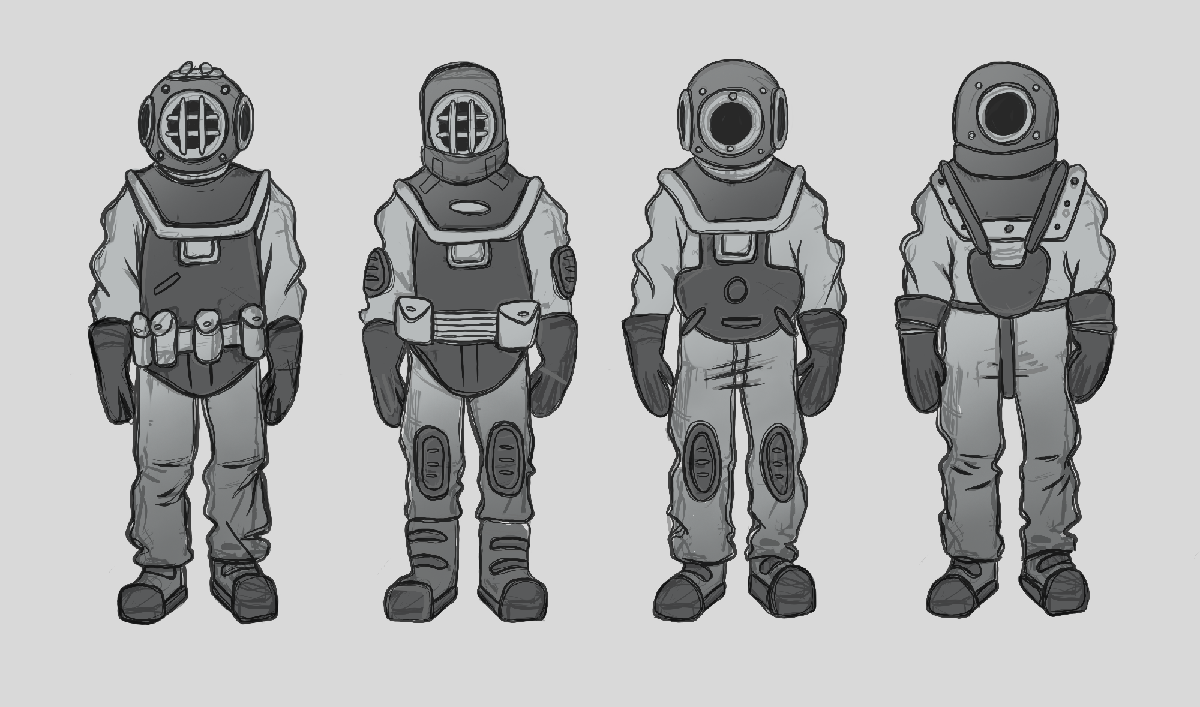
\includegraphics[width=10cm]{assets/CONCEPT_PROTAGONISTE}
\end{frame}

\begin{frame}{Concept Art des ennemis}
    \centering
    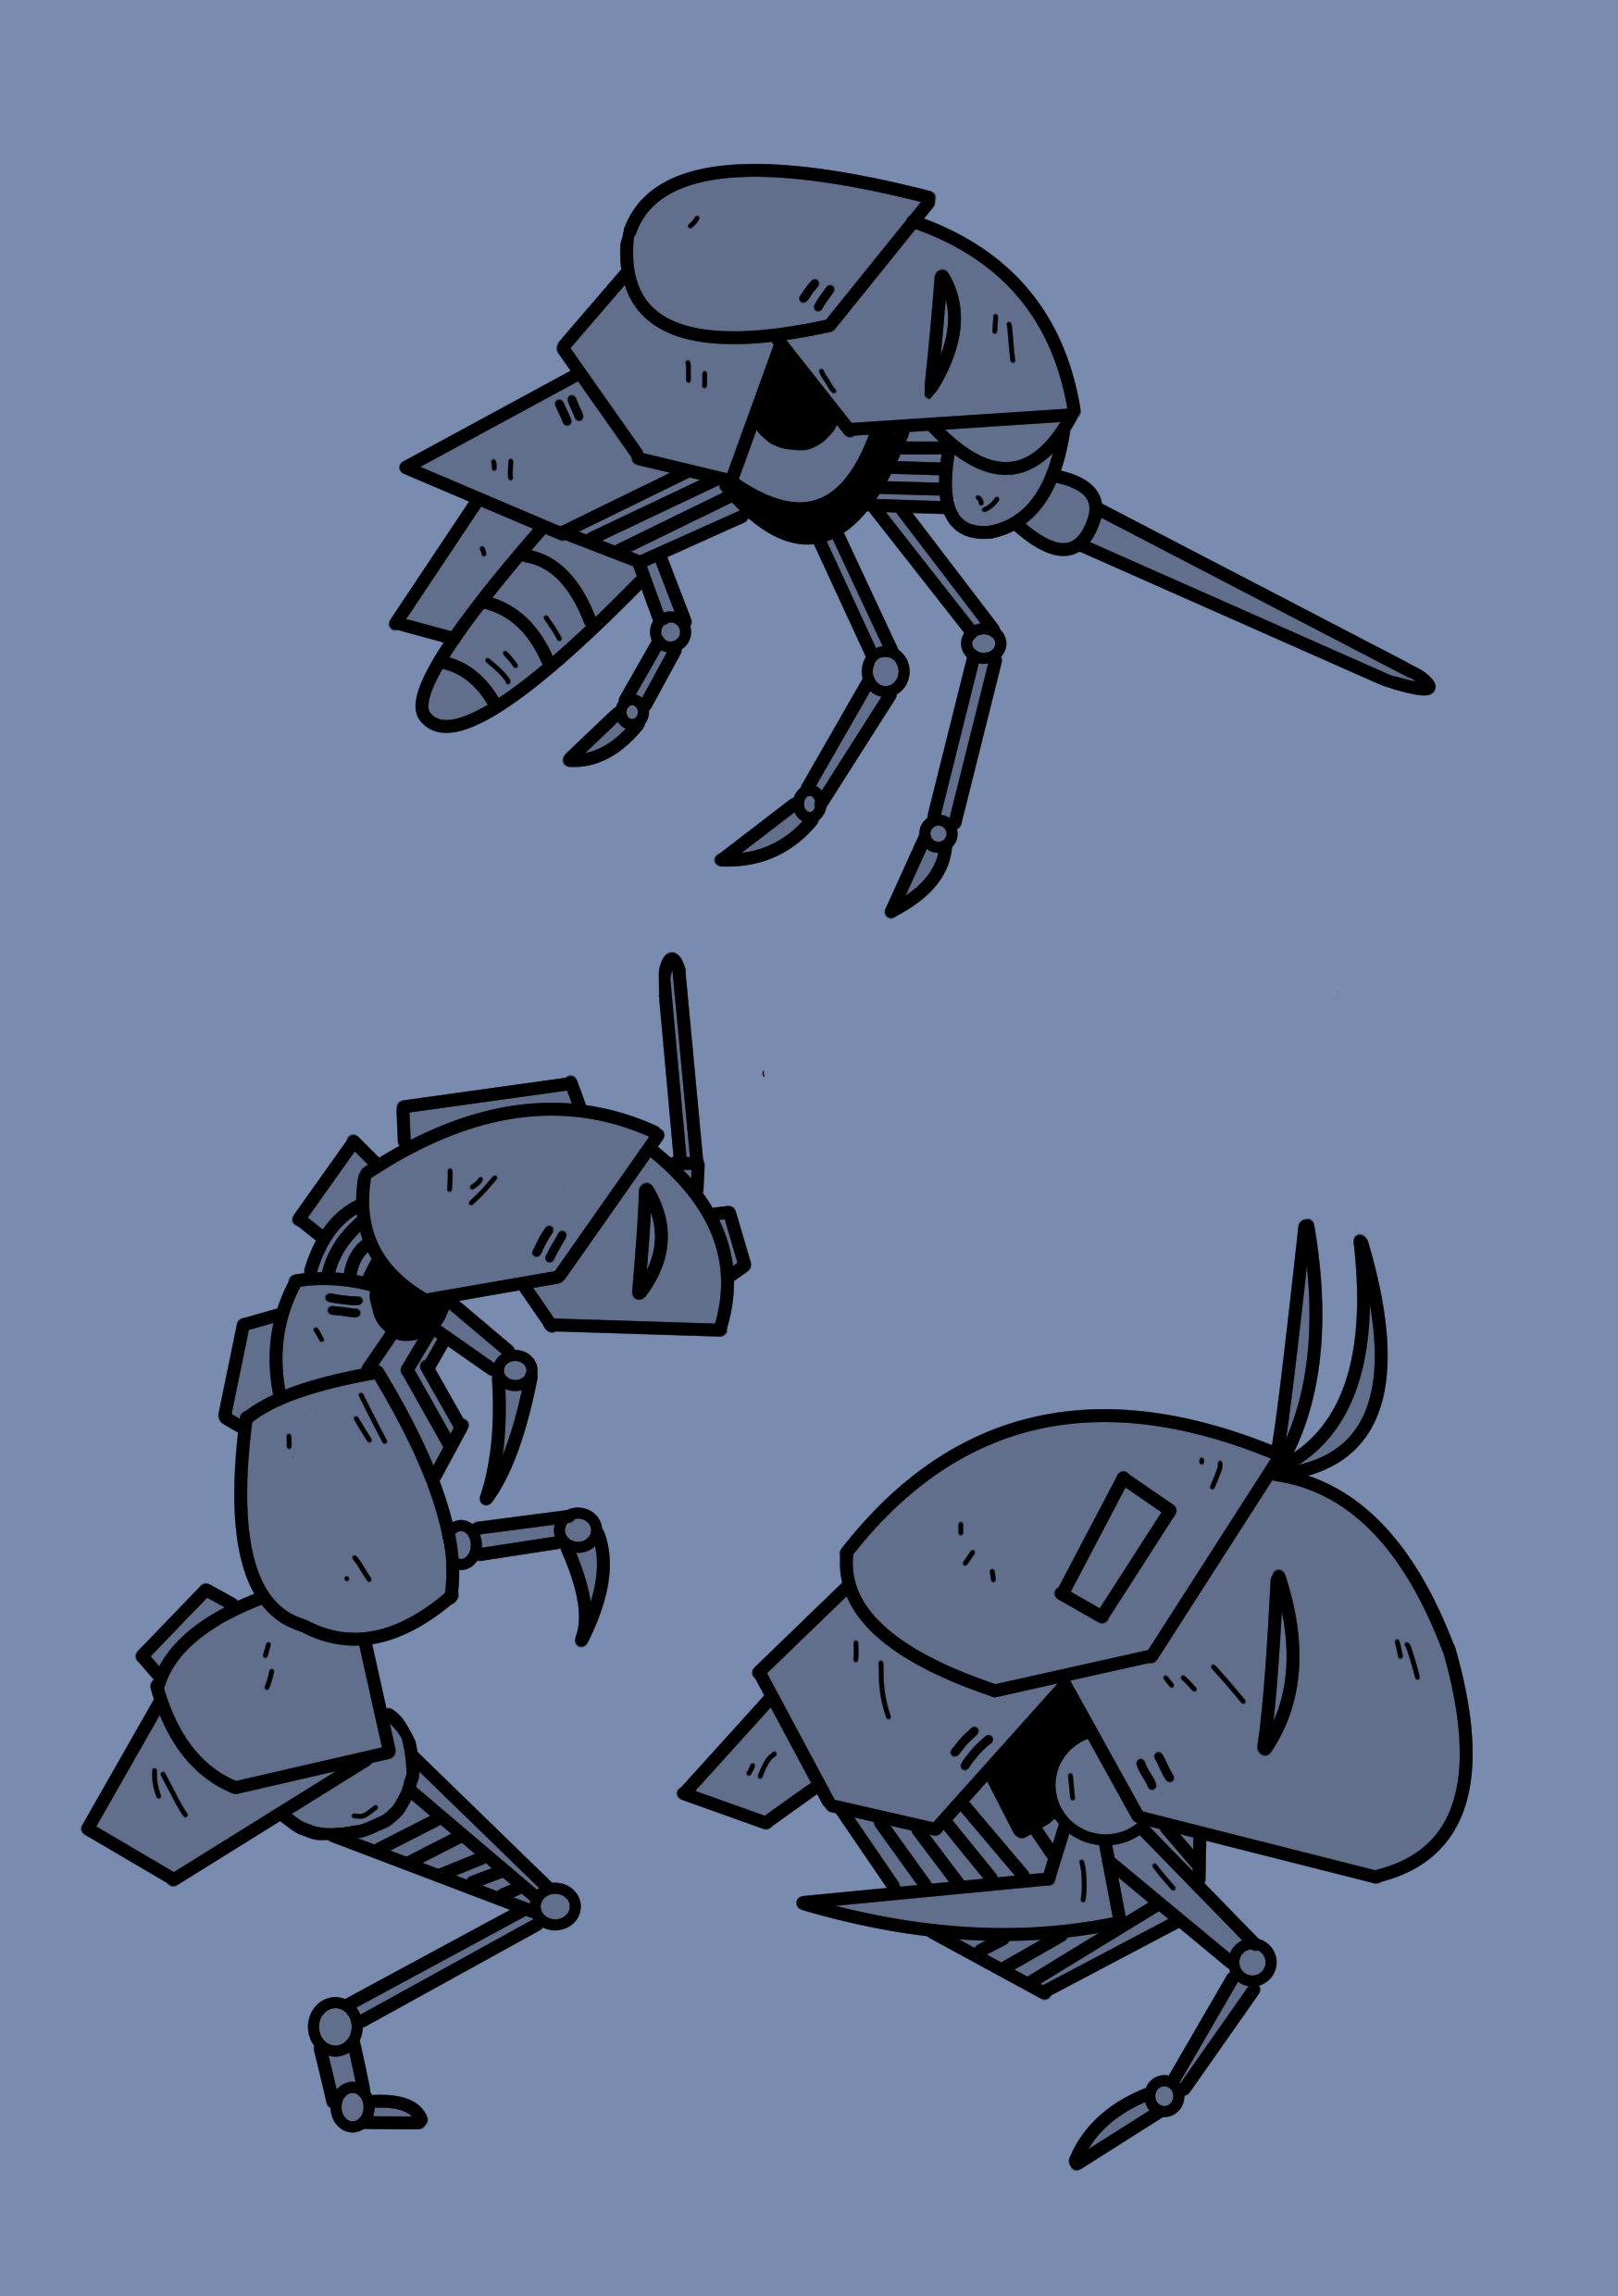
\includegraphics[height=7cm]{assets/02}
\end{frame}

\begin{frame}{Concept Art in game}
    \centering
    \includegraphics[width=10cm]{assets/002MAX}
\end{frame}

\begin{frame}{Concept platformer}
    \centering
    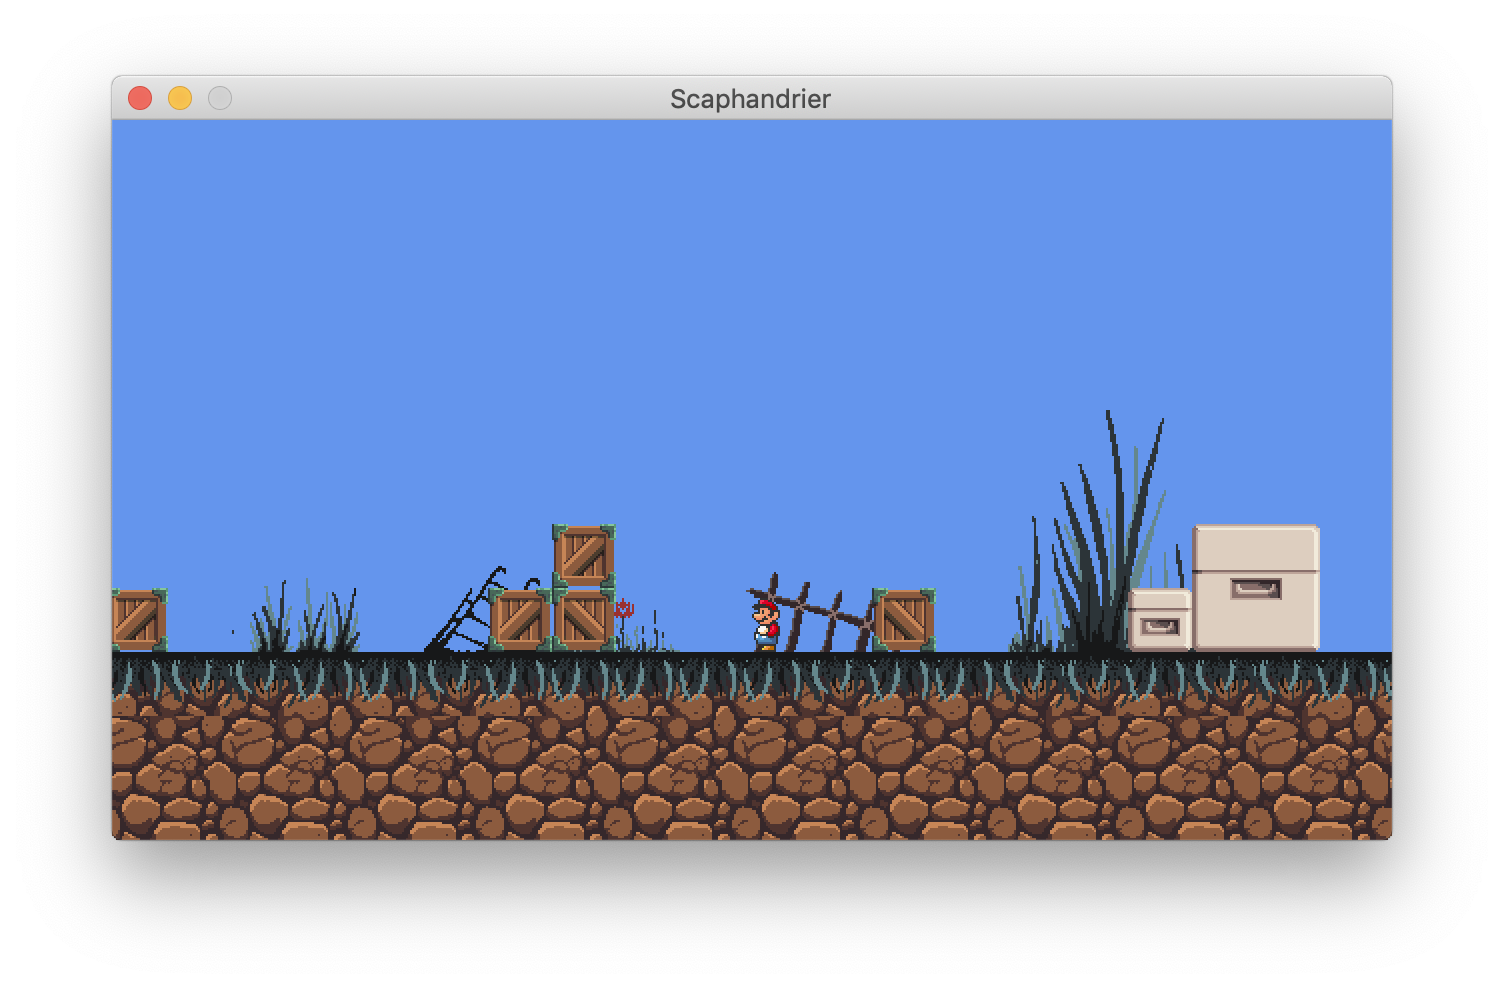
\includegraphics[width=10cm]{assets/unknown}
\end{frame}

\begin{frame}{Résultat}
    \centering
    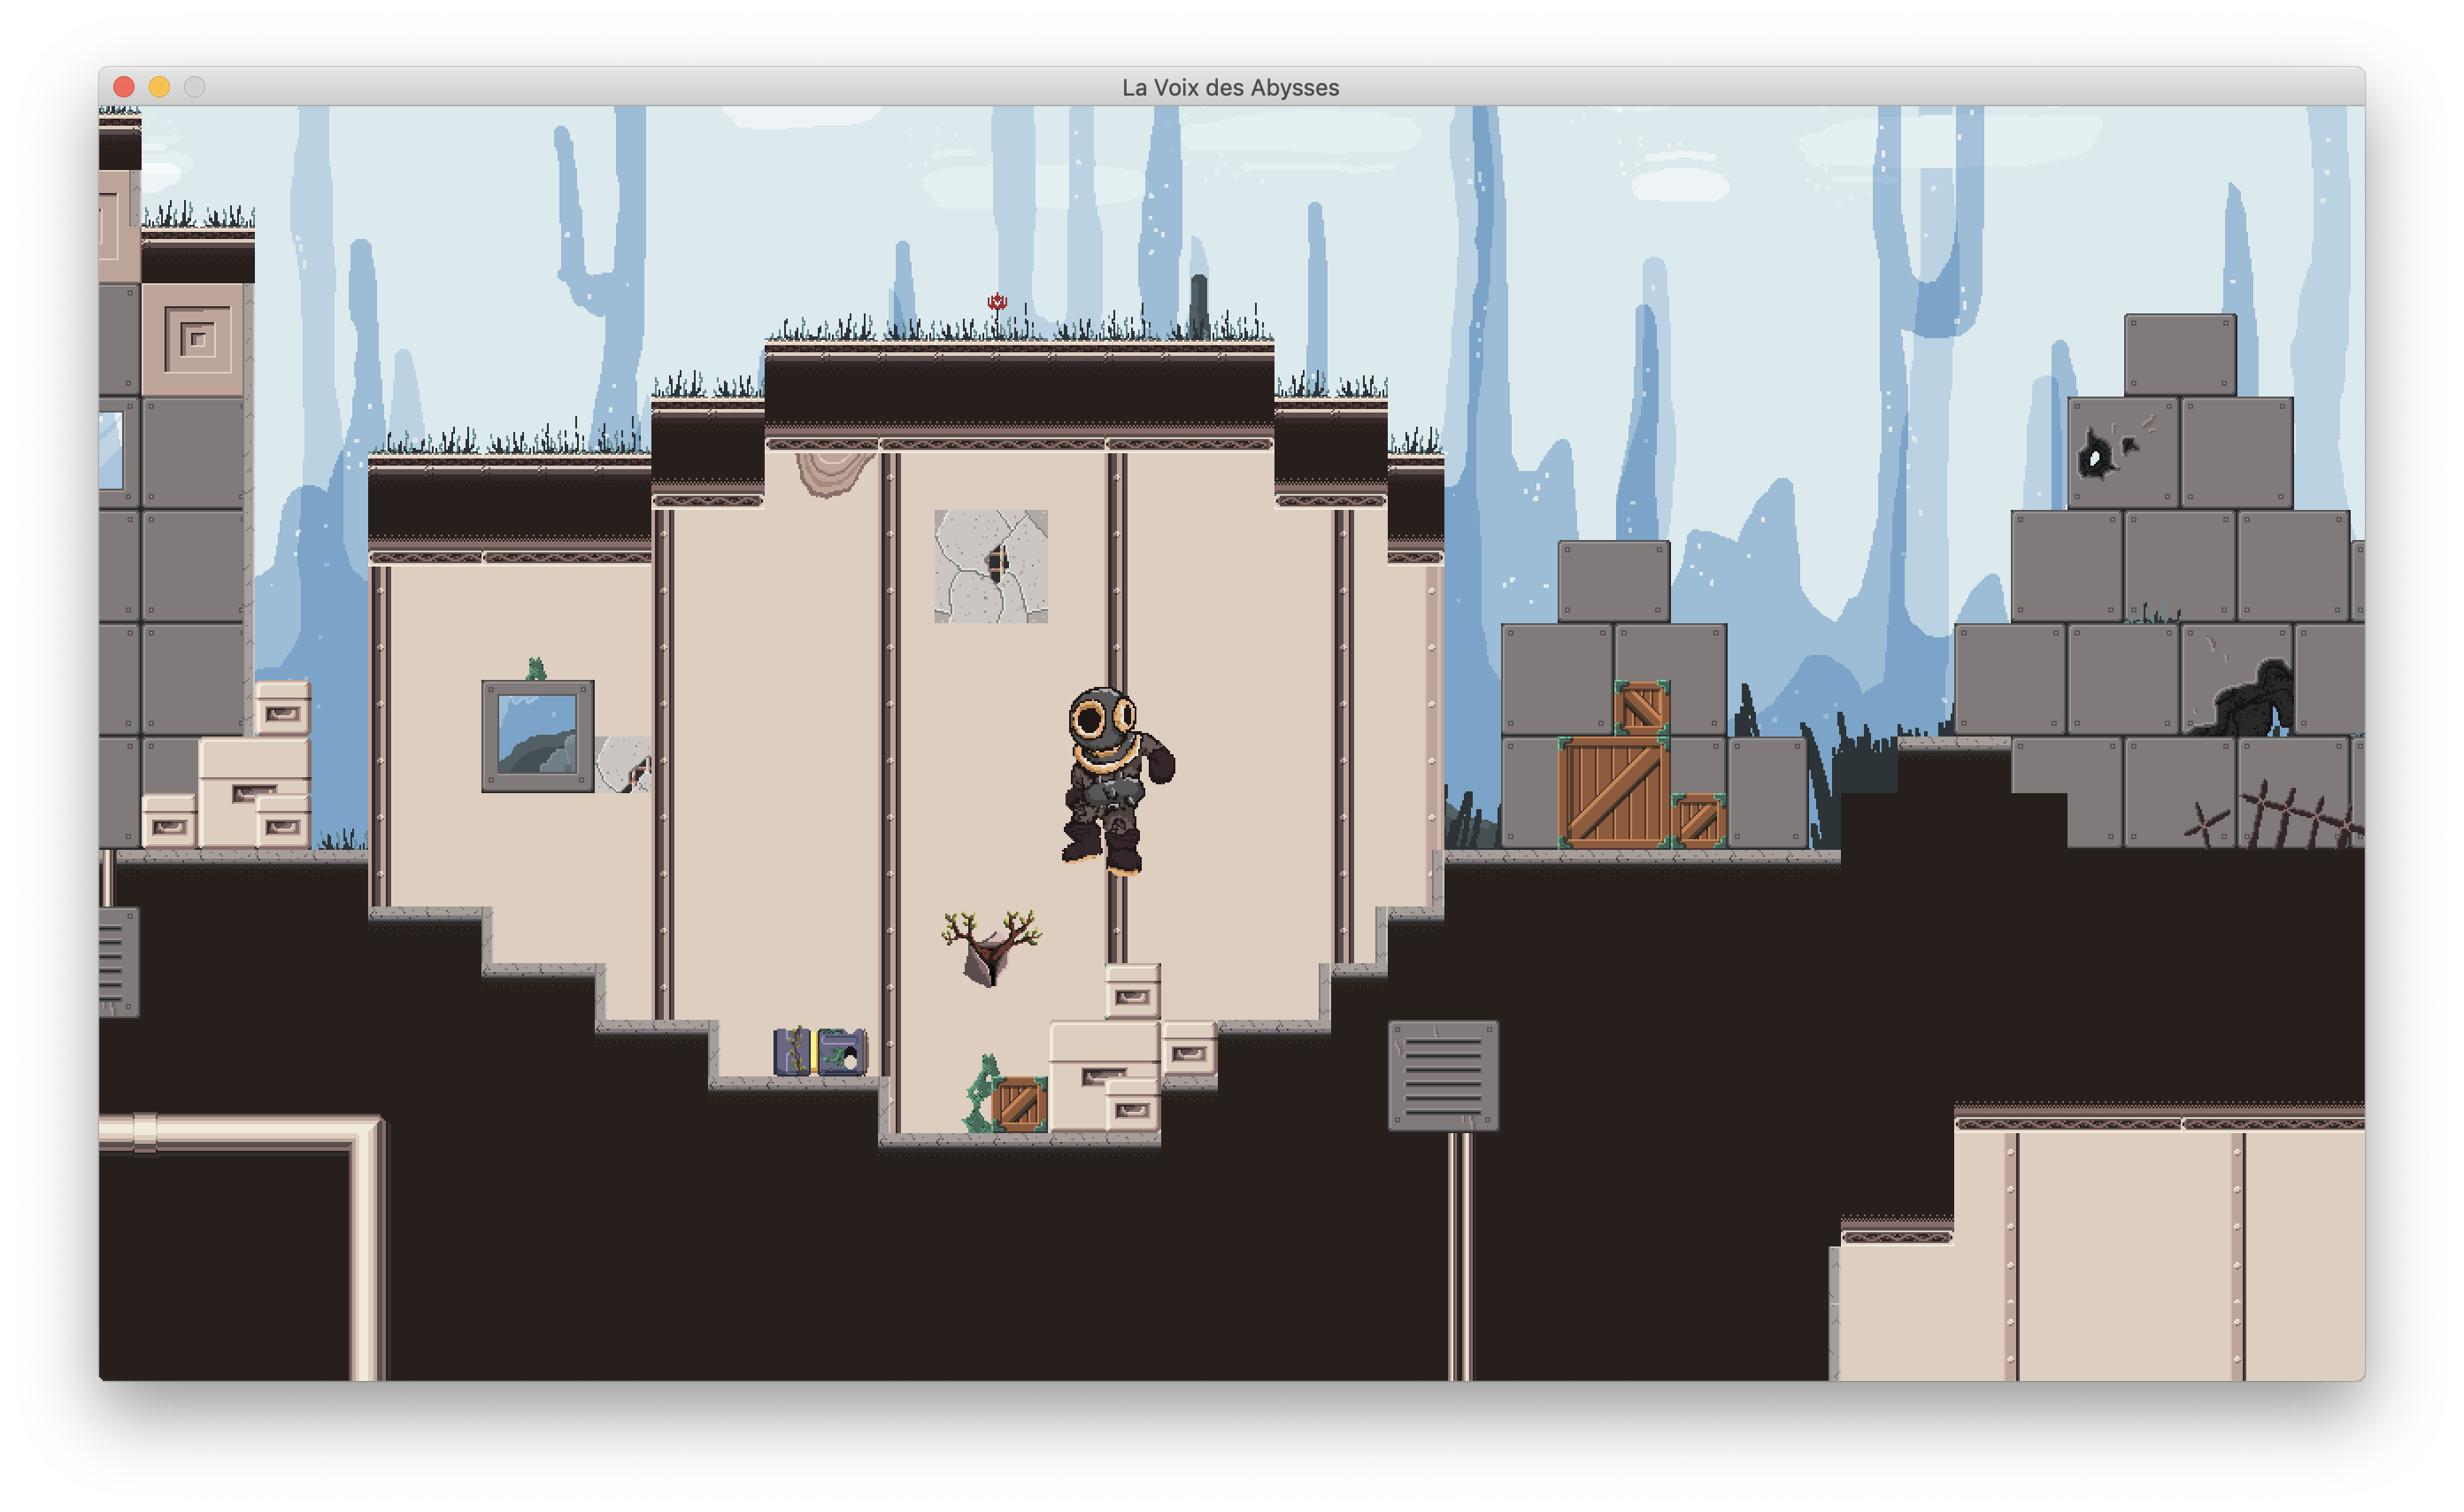
\includegraphics[width=10cm]{assets/ingame}
\end{frame}

\section{Technique}

\subsection{Outils}

\begin{frame}{Framework MonoGame}
  
\end{frame}

\begin{frame}{Visual Studio}
  
\end{frame}

\begin{frame}{Tiled}
  
\end{frame}

\subsection{Fonctionnement du jeu}

\begin{frame}{Organisation générale}
    \centering
    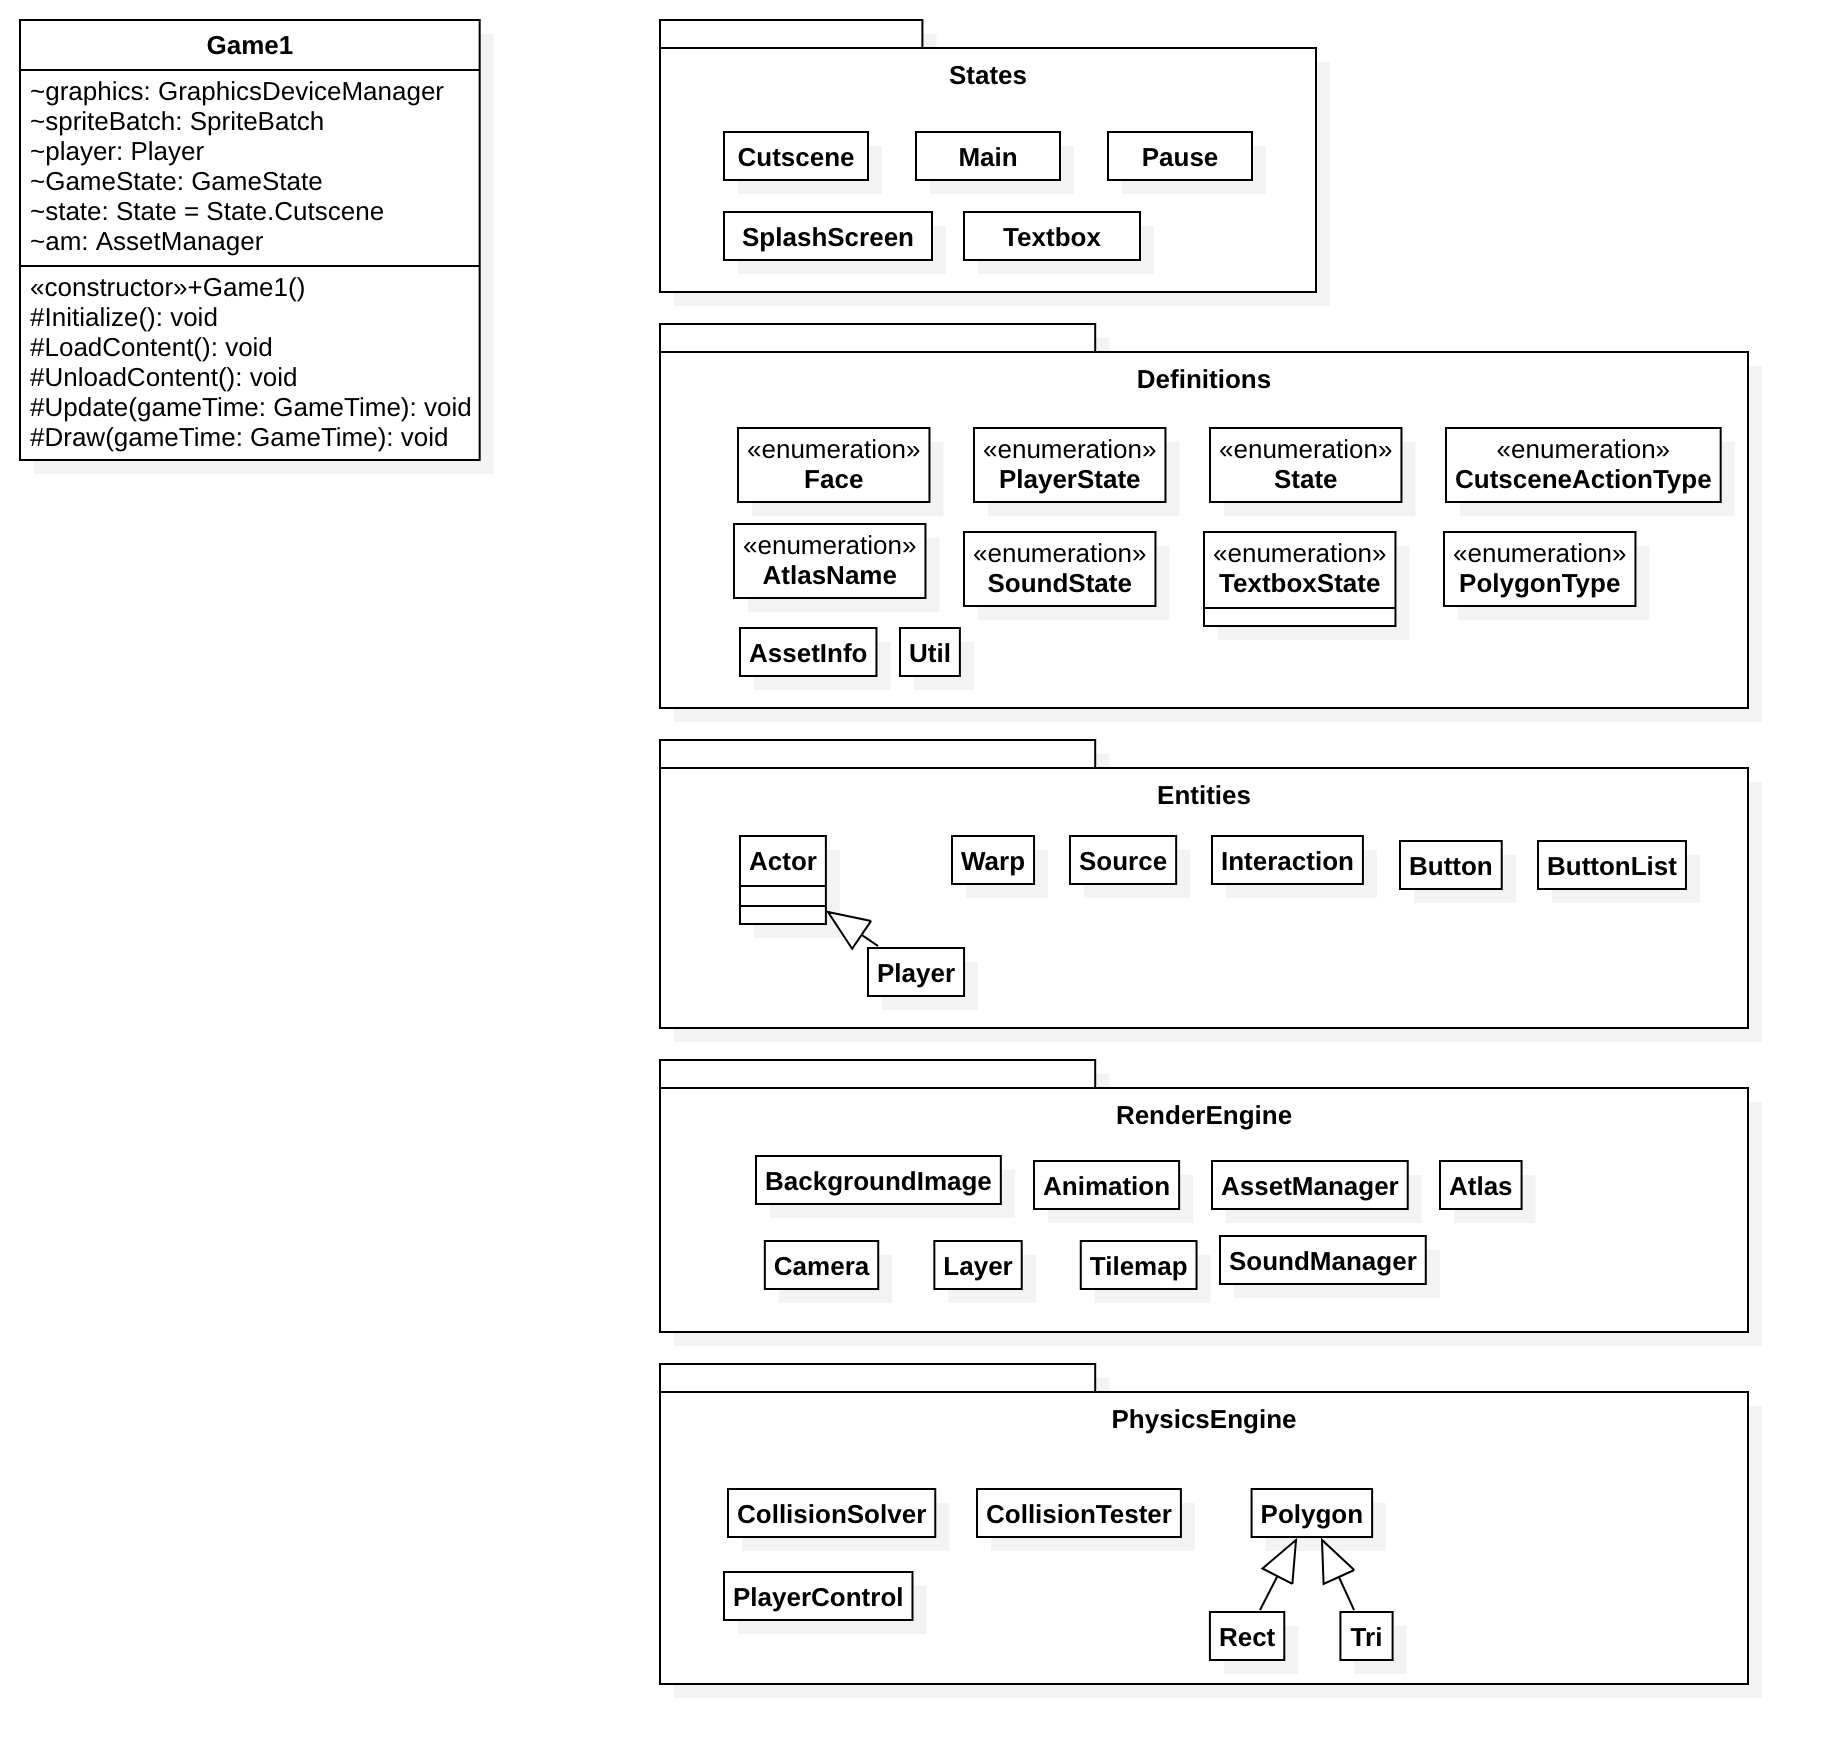
\includegraphics[width=9cm]{assets/uml}
\end{frame}

\begin{frame}{Game1.cs : Update()}
    \centering
    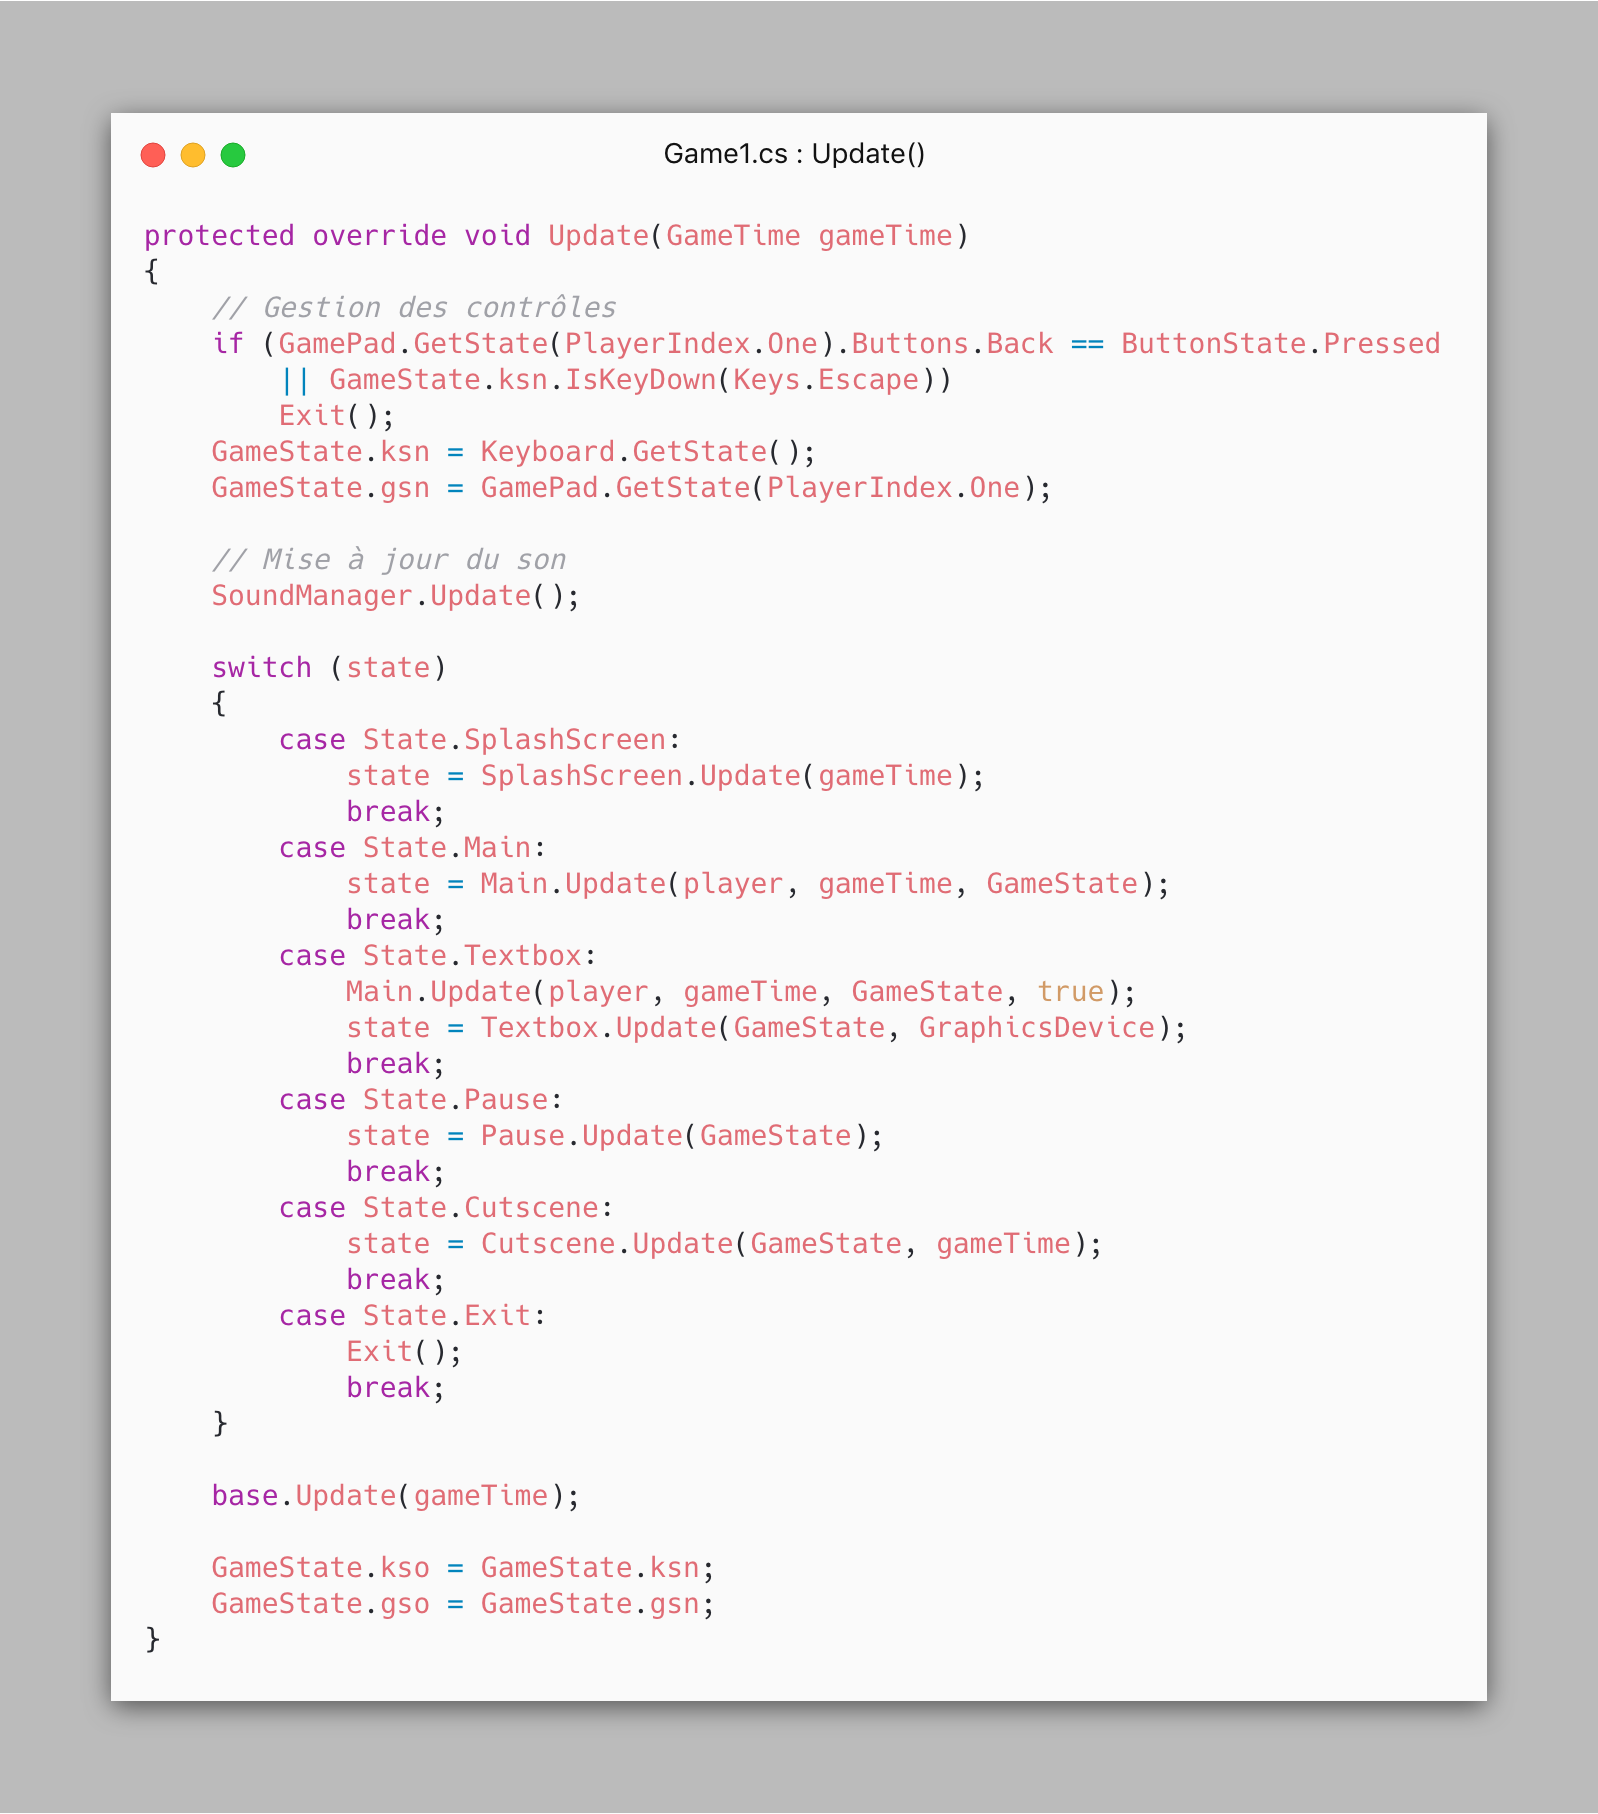
\includegraphics[width=7cm]{assets/game1update}
\end{frame}

\begin{frame}{Game1.cs : Draw()}
    \centering
    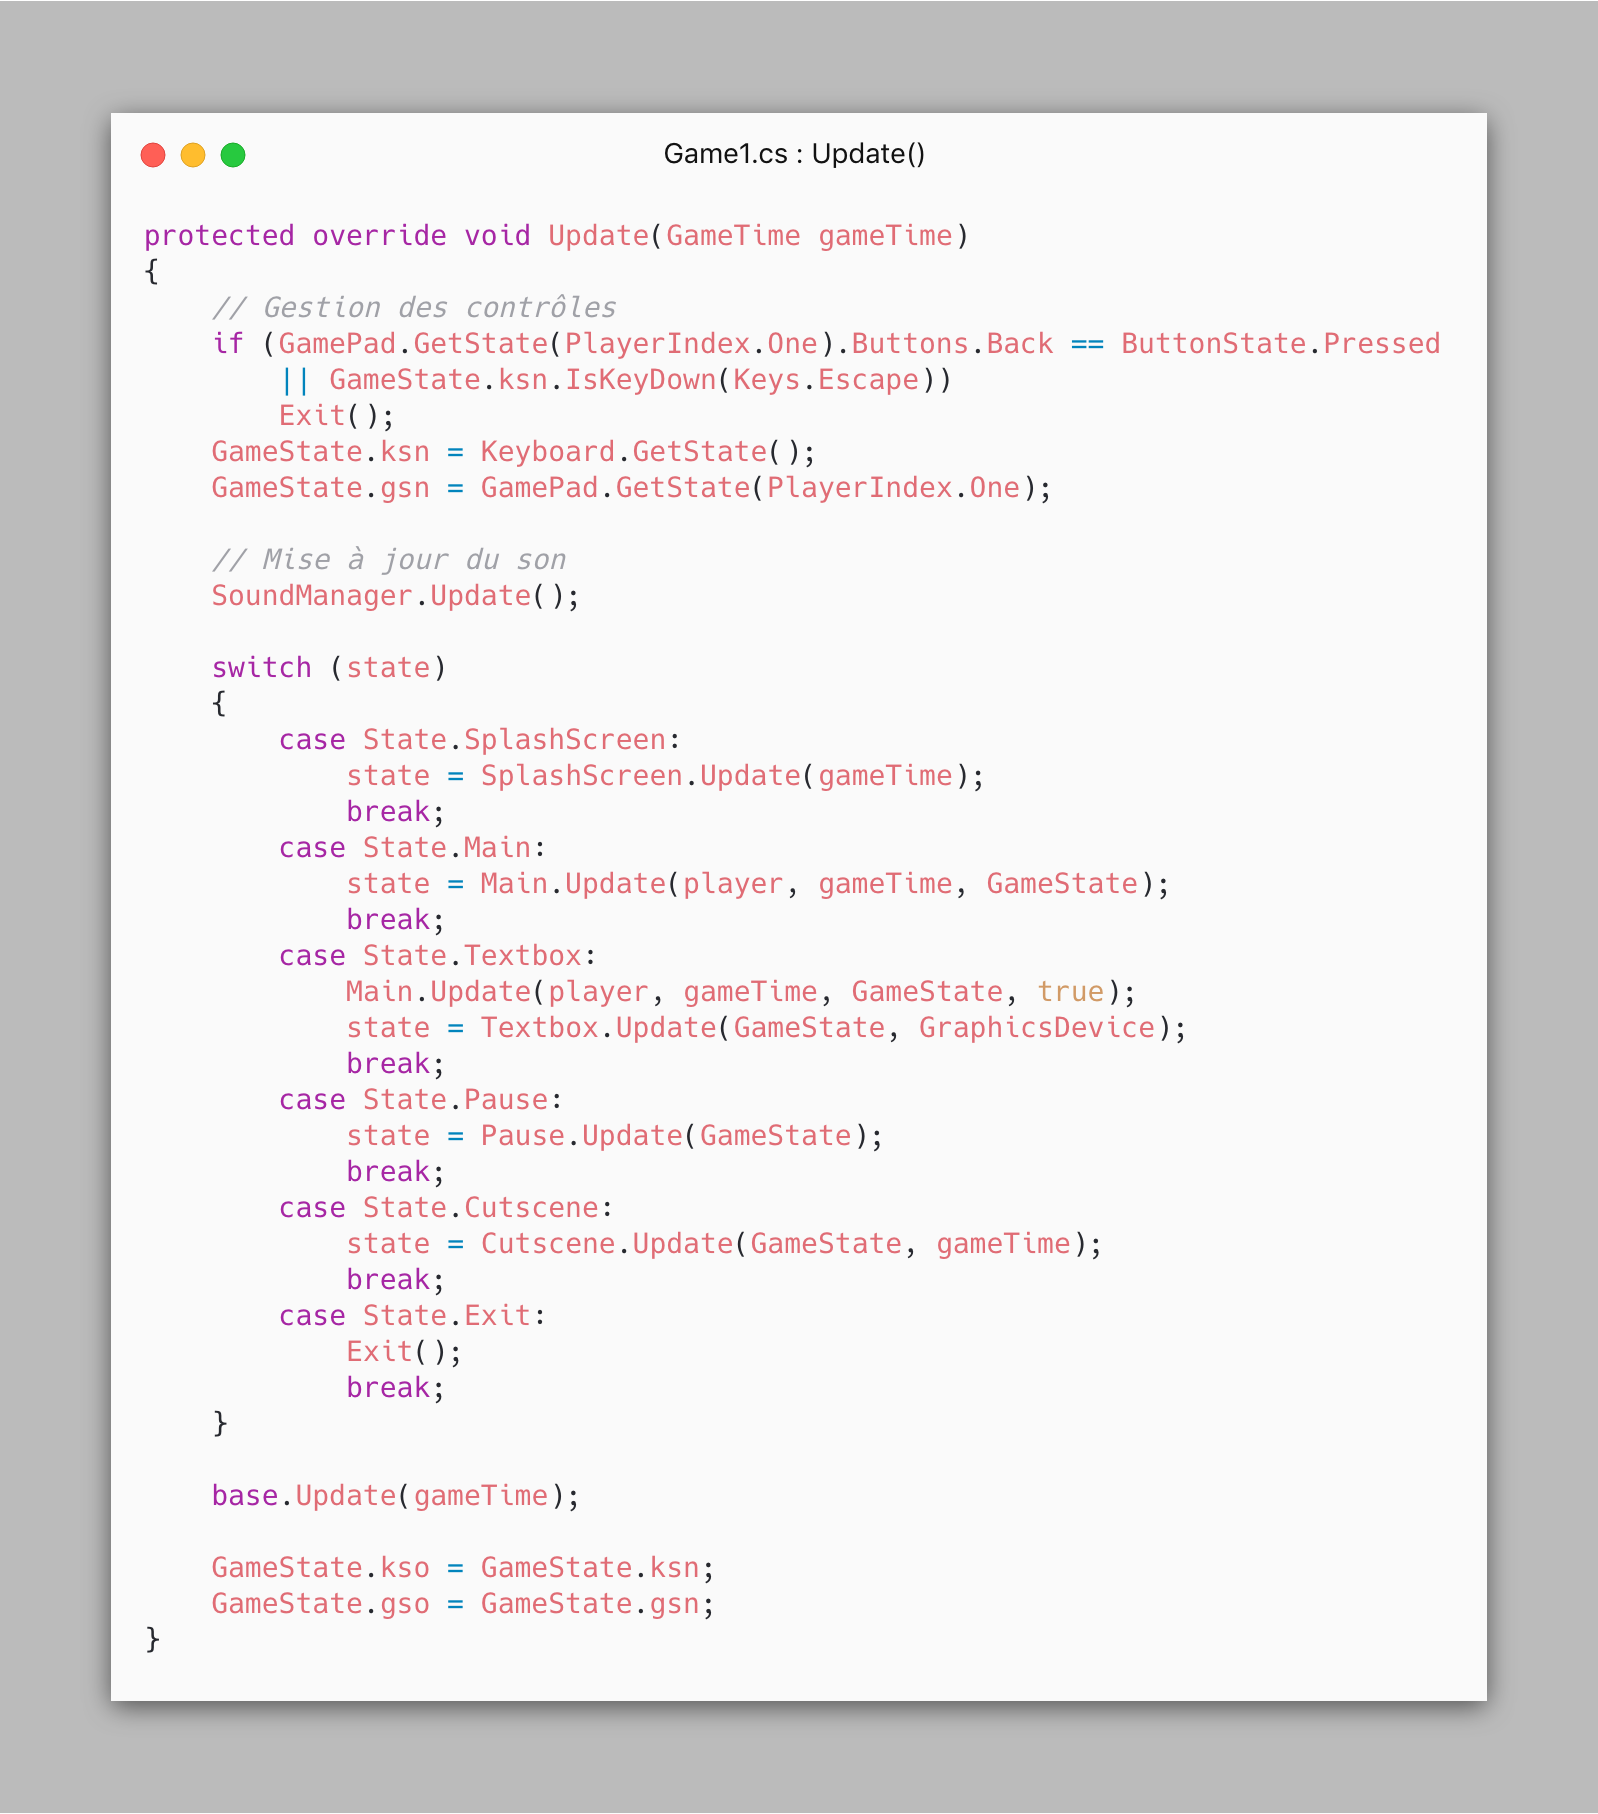
\includegraphics[width=7cm]{assets/game1update}
\end{frame}

\begin{frame}{Cutscene.cs : traitement d'une cinématique}
    Décomposition d'une cinématique en différentes actions
    
    \begin{itemize}
        \item Background : affichage d'images
        \item Text : affichage texte
        \item NewPage : nouvelle page d'écriture
        \item Wait : temps d'attente
        \item Sfx : effet sonore
        \item Bgm : musique d'ambiance
        \item State : nouvel état
    \end{itemize}
\end{frame}

\begin{frame}{Cutscene.cs : traitement d'une cinématique}
    Récupération des actions : 

    \centering
    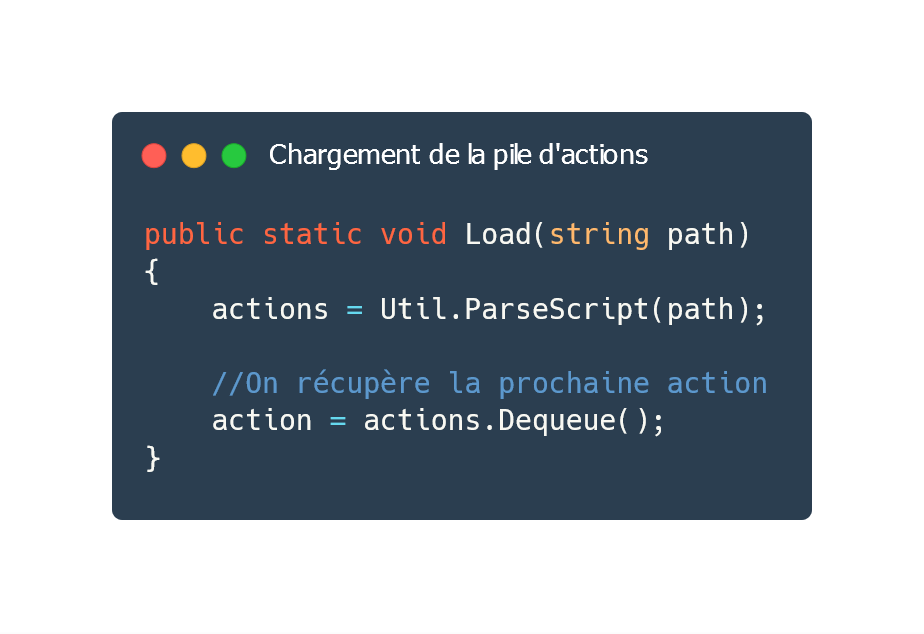
\includegraphics[width=7cm]{assets/pile_cutscene}
\end{frame}

\begin{frame}{Textbox.cs}
  
\end{frame}

\begin{frame}{Atlas.cs}
  
\end{frame}

\begin{frame}{Tilemap.cs}
  
\end{frame}

\begin{frame}{Le son : dans Tiled}
    \centering
    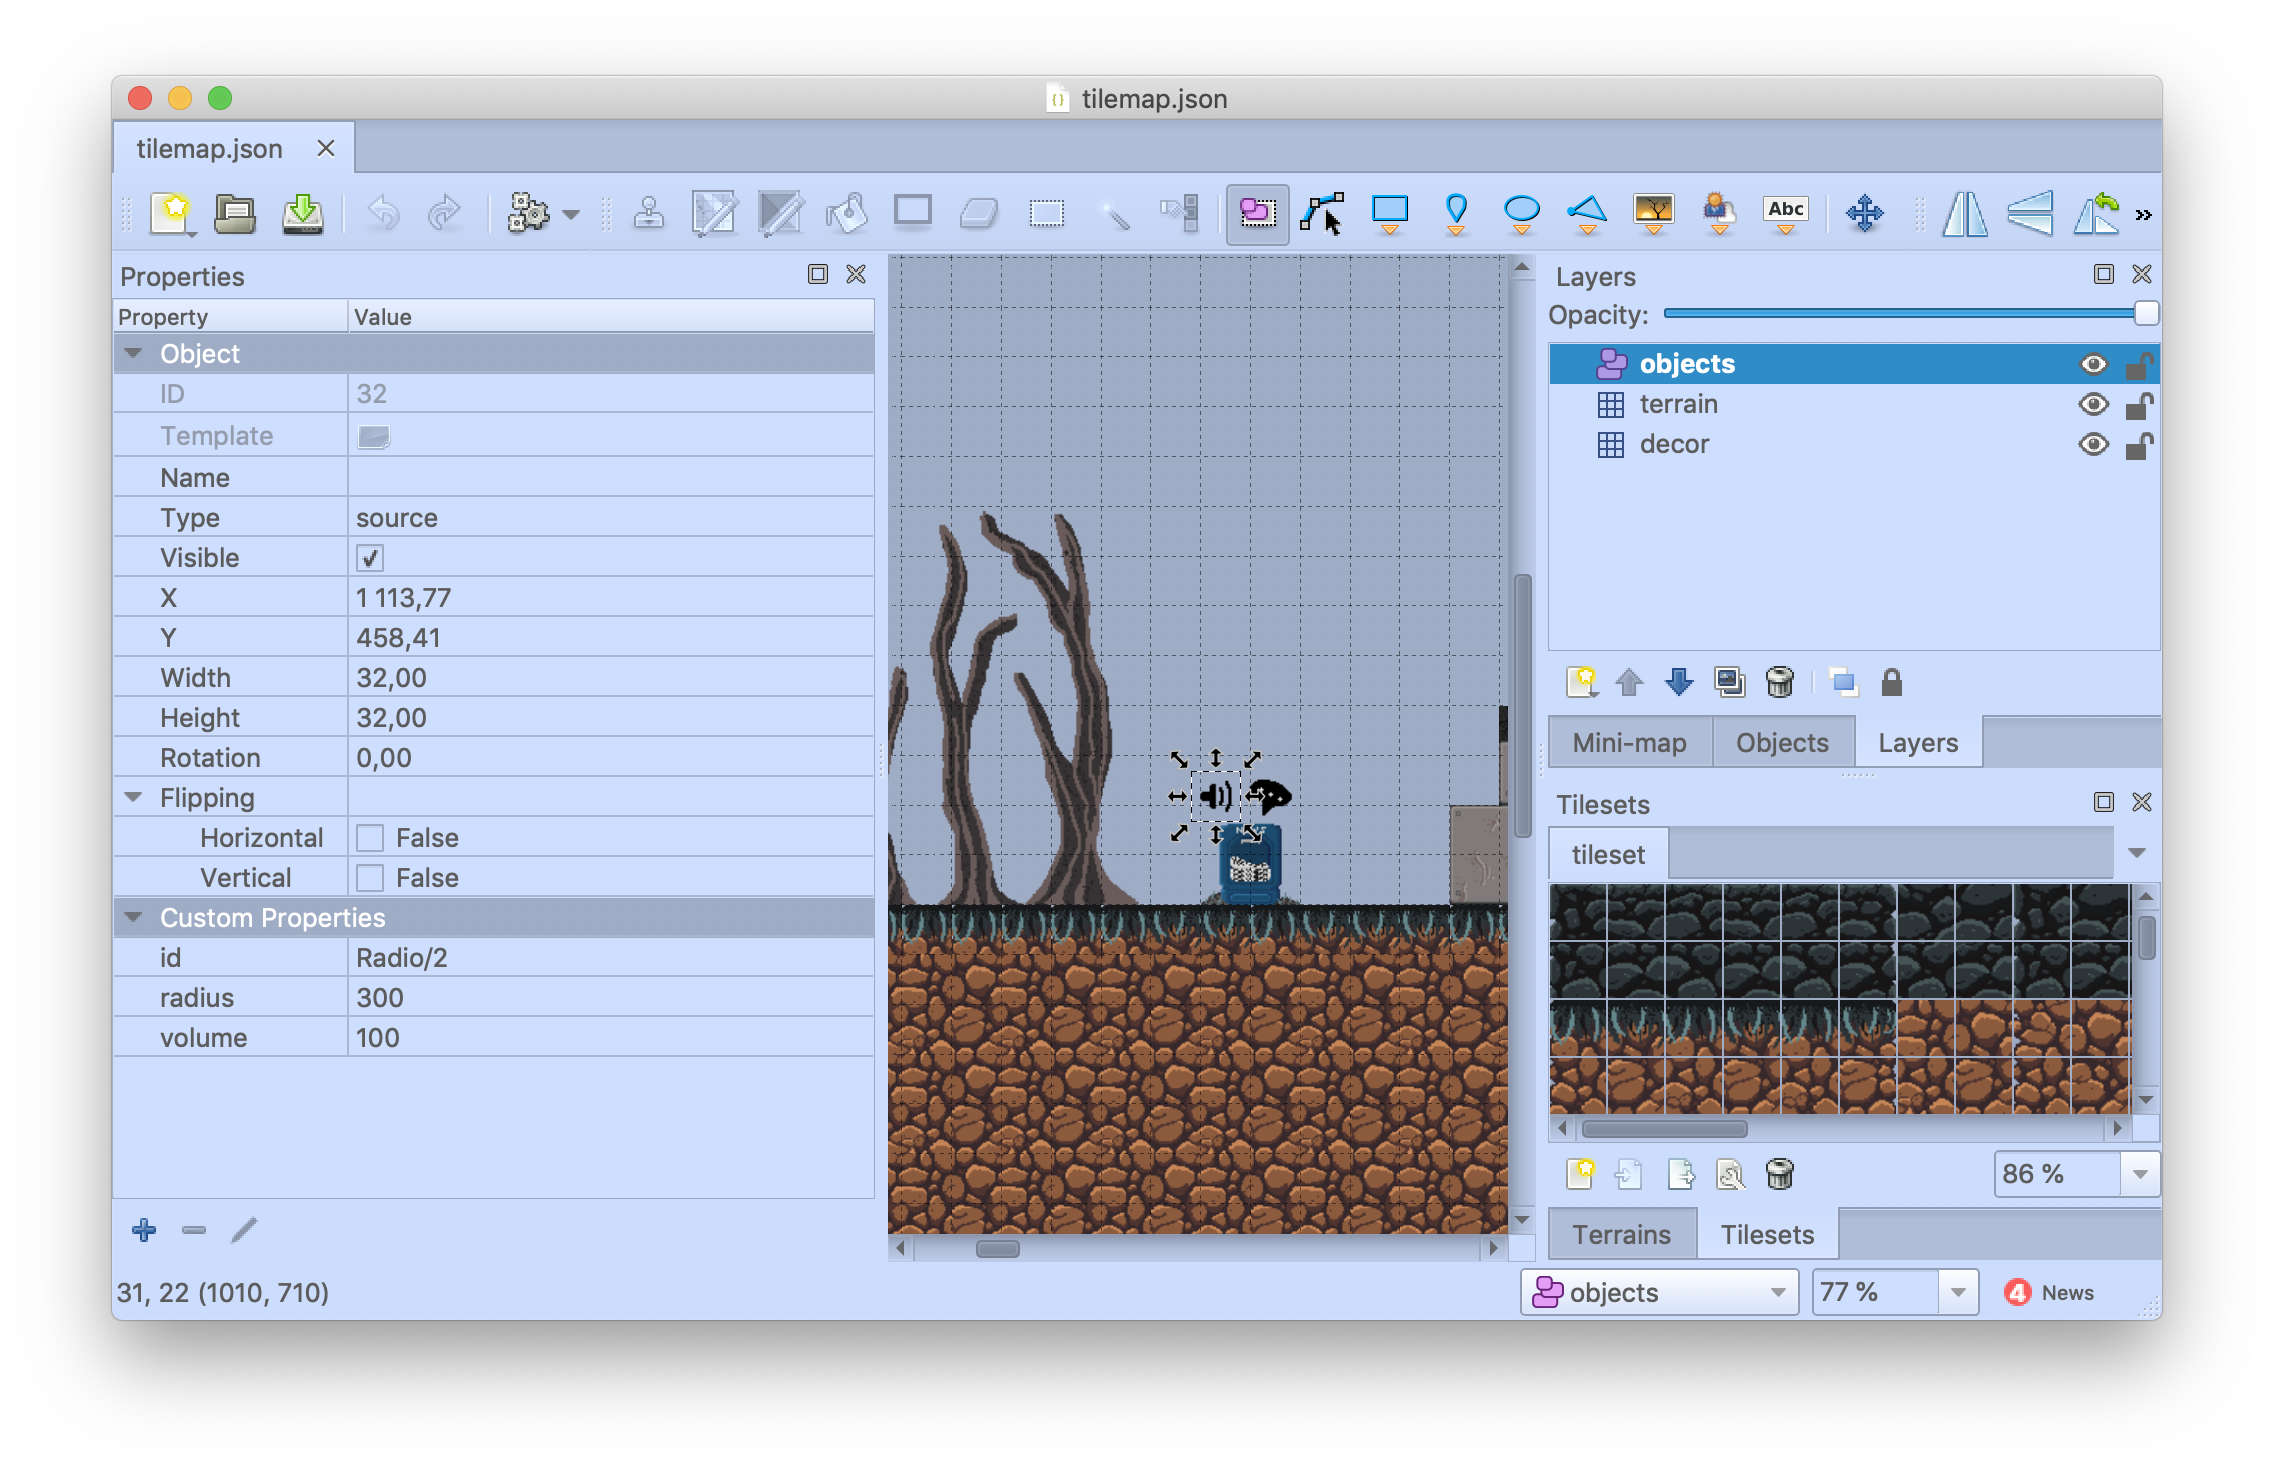
\includegraphics[width=10cm]{assets/tiledSon}
\end{frame}

\begin{frame}{Le son : JSON généré}
    \centering
    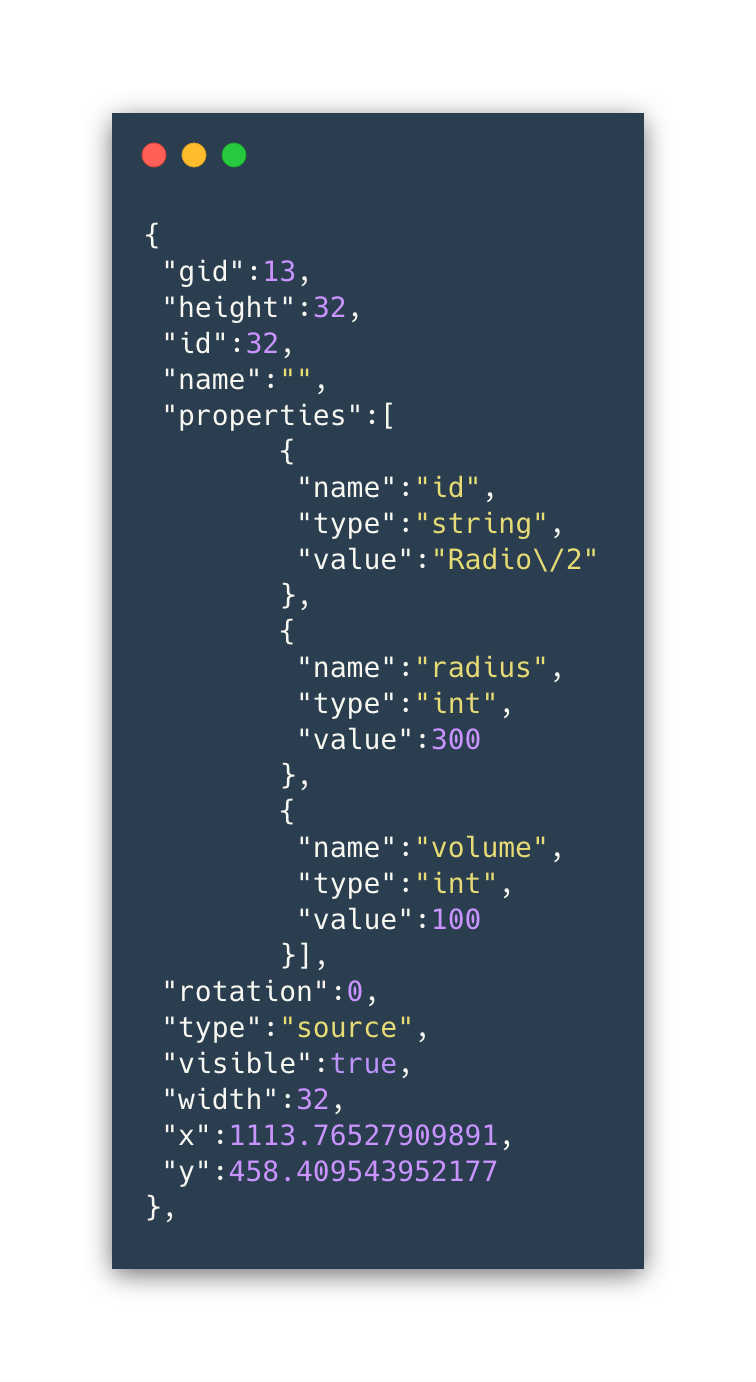
\includegraphics[width=4cm]{assets/jsonSource}
\end{frame}

\section{Perspectives}

\begin{frame}{Finir le projet}
  
\end{frame}

\end{document}